\documentclass[paper=a4, english, ngerman, romanian]{scrartcl}

\usepackage[a4paper,left=2cm,right=2cm,top=2.5cm,bottom=3cm]{geometry}
\usepackage[ngerman]{babel}
\usepackage{tabularx}
\usepackage[utf8]{inputenc}
\usepackage{multirow}
\usepackage{listings}
\usepackage{graphicx}
\usepackage[absolute]{textpos}
\usepackage{amsmath}
\usepackage{mathtools}
\usepackage{amssymb}
\usepackage{dsfont}
\usepackage{wasysym}
\usepackage{enumitem}
\usepackage{stmaryrd}

\parindent 0pt
\lstset{basicstyle={\ttfamily\scriptsize}, tabsize=4}
\begin{document}

\begin{titlepage}
	\title{Datenbanksysteme SS17: Projekt, 3. Iteration}	
	\subtitle{Dozentin: Agnes Voisard}
	\author{Bernadeta Chisarau, Dor Cohen, Mihai Renea}
	\date{\normalsize \today}
\end{titlepage}

\maketitle								% Erstellt das Titelblatt
\vspace*{-8cm}							% rückt Logo an den oberen Seitenrand
\makebox[\dimexpr\textwidth+1cm][r]{	%rechtsbündig und geht rechts 1cm über Layout hinaus
	
\includegraphics[width=0.4\textwidth]{src/fu_logo} % fügt FU-Logo ein
}

\vspace{7cm}							% Abstand
\rule{\linewidth}{0.8pt}				% horizontale Linie
	\section{Clusteranalyse}
		Für die Clusteranalyse haben wir den K-Means Algorithmus mithilfe der java-ml Library eingesetzt. Der Algorithmus partitioniert die Menge der Hashtags in 10 Clusters, wo jedes Hashtag ein 2-dimensionales Vektor mit den folgenden Metriken ist:
		\begin{itemize}
			\item Hashtag-Wichtigkeit -- als Durchschnitt der Wichtigkeitswerten aller Tweets, die Hashtag $h$ enthalten.\\
			Wichtigkeit $W_T(t)$ eines Tweets $t$:\\
			\begin{equation*}
				W_T(t) = ^4\sqrt{\frac{t_{favorites\ count} + t_{retweet\ count}}{2}}
			\end{equation*}
			Wichtigkeit $W_H(h)$ eines Hashtags h:
			\begin{equation*}
				W_H(h) = \frac{\sum_{t \in T} W_T(t)}{|T|}
			\end{equation*}
			Wo $T$ die Menge der Tweets, die Hashtag $h$ enthalten.
			
			\item Hashtag-Occurence -- wie oft ein Hashtag insgesamt aufgetaucht hat.
		\end{itemize}
		
		Anschließend speichern wir die neu-erzeugten Informationen in einer neuen Tabelle, \textit{hashtag}. Damit kann man für die Visualisierung die gebrauchten Werte einfach ablesen. Dadurch entsteht die aktuelle DB-Schema:
		
		\begin{center}
			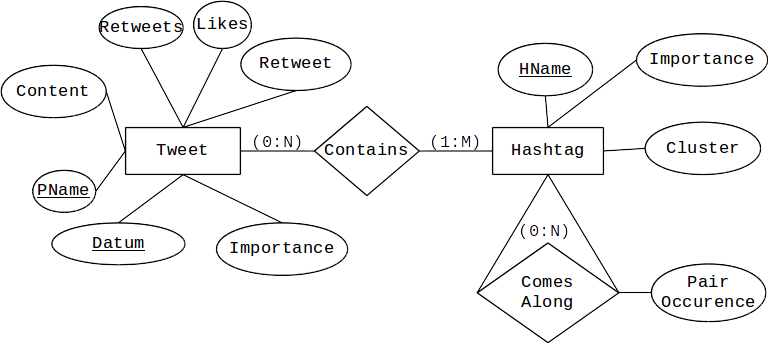
\includegraphics[scale=0.6]{src/MinMax_Diagram}
		\end{center}
		
		


\end{document}
